%! Author = matteomagnini
%! Date = 05/03/25

%----------------------------------------------------------------------------------------
\chapter[Fairness through SKI]{Fairness through \gls{SKI}}
\label{ch:fairness-through-ski}
\minitoc
%----------------------------------------------------------------------------------------

\Gls{AI} has transformed various aspects of modern society.
%
With recent groundbreaking advancements, its applications are expected to grow exponentially.
%
However, the issue of fairness has become a significant concern.
%
When \gls{AI} systems are deployed without adequate safeguards, they risk perpetuating or amplifying existing social biases.
%
For example, a recruitment system trained on historical data dominated by male hires may discriminate against female applicants, reinforcing gender bias~\cite{kochling2020genderbias}.
%
To address such challenges, numerous techniques have been developed to mitigate bias in \gls{AI}.
%
Among these, regularization-based fairness techniques have gained prominence for balancing fairness and predictive performance.
%
Regularization, initially introduced to prevent overfitting, involves adding a penalty term to the loss function during training.
%
Recently, it has been extended to promote fairness by incorporating penalties derived from fairness constraints~\cite{kamishima2011fairness}.
%
These methods aim to reduce the dependence of predictions on sensitive attributes, such as gender, making them effective for bias mitigation during optimization steps like \gls{SGD} in \gls{ML} algorithms.
%

\section{Background}\label{sec:fairness-background}
%
We provide a brief but comprehensive overview of fairness in \gls{ML} to understand our contributions without delving into the extensive literature on the topic.
%
The section is organised as follows.
%
In \Cref{subsec:fairness-motivations}, we discuss the motivations for fairness in \gls{ML} and how it is related to \gls{SKI}.
%
In \Cref{subsec:fairness-metrics}, we introduce common group fairness metrics used in the literature, along with some of their limitations that motivate the development novel metrics.
%
Finally, in \Cref{sec:fauci}, we present our contributions to fairness in \gls{ML}.


\subsection{Motivations}\label{subsec:fairness-motivations}
%
\Gls{ML} models can inherit and amplify biases present in the dataset \(D\).
%
For instance, if \(D\) contains features related to gender or race, and the data is not equally distributed across these groups, biases may arise.
%
This often occurs in datasets about hiring decisions, where historical data may reflect fewer non-male or non-white candidates.
%
A supervised model \(H\), trained on such a dataset to predict a target feature \(Y\), might incorrectly learn that gender or race influences the prediction.
%
If the predictions of \(H\) are used for decision-making, such as hiring or loan approvals, the model may discriminate against certain groups.
%
In this case, the model is said to be biased, as it replicates patterns of past discrimination.

%
Fairness interventions can mitigate these biases and are applied at different stages of the \gls{ML} workflow.
%
In the literature, these methods are categorized as:
%
\begin{itemize}
    \item \textit{Pre-processing methods}, which modify the dataset \(D\) to reduce bias before training;
    %
    \item \textit{In-processing methods}, which adjust the learning algorithm \(A\) to enforce fairness during training;
    %
    \item \textit{Post-processing methods}, which modify the predictions of the model \(H\) to achieve fairness after training.
\end{itemize}

%
A critical prerequisite for fairness interventions is the ability to measure fairness.
%
Fairness metrics quantify the extent of bias in a dataset or model and evaluate the effectiveness of mitigation techniques.
%
Formally, a fairness metric is a function that takes data as input and returns a numerical score.
%
The input data can be a dataset \(D = (X, Y)\) or the predictions \(h(X)\) of a model on \(D\).
%
A lower score typically indicates higher bias, while a higher score reflects greater fairness.

%
Numerous fairness metrics have been proposed, differing in the type of data they accept and their interpretation of fairness or bias.
%
These metrics are often categorized based on the fairness notion they adhere to~\cite{mehrabi2022fairness}.
%
The two most common notions are \textit{group fairness} and \textit{individual fairness}.


\paragraph{Group fairness}\label{par:group-fairness}
%
Group fairness ensures that distinct groups of individuals, defined by sensitive attributes, are treated equally.
%
Sensitive attributes, denoted as \( S \subset X \), are features such as \emph{gender}, \emph{race}, \emph{age}, or social status, which partition the dataset \( D \) into protected groups.
%
These groups can be defined by a single sensitive attribute, e.g., the group of women identified by a specific value of the \textit{gender} feature, or by a combination of attributes, e.g., the group of Black women identified by both \textit{gender} and \textit{race}.
%
The principle of group fairness is commonly evaluated by measuring the correlation between sensitive attributes \( S \) and the target variable \( Y \).
%
For instance, if \( Y \) represents loan approval outcomes and \( S \) represents the applicant's race, group fairness metrics assess whether the approval rates are consistent across racial groups.
%
Such metrics are crucial for identifying and addressing biases in decision-making processes.


\paragraph{Individual fairness}\label{par:individual-fairness}
%
Individual fairness ensures that similar individuals receive similar treatment.
%
The simplest approach to individual fairness is \emph{fairness through awareness}.
%
This method relies on a distance metric \(\delta : X \times X \to \mathbb{R}\) in the input space (e.g., Euclidean distance).
%
It requires that if two individuals \(x_1\) and \(x_2\) are similar up to a threshold \(\epsilon\), i.e., \(\delta(x_1, x_2) < \epsilon\), then their corresponding target values \(y_1\) and \(y_2\) should also be similar.
%
In practice, model predictions \(h(x_1)\) and \(h(x_2)\) are compared instead of true labels, and fairness scores are computed by averaging the differences in predictions for similar instances.
%
Another approach is \emph{fairness through unawareness}, which requires that sensitive attributes are not used by the model during training or prediction.
%
This can be achieved by removing sensitive features from the dataset or ensuring the model does not rely on them.
%
Fairness scores in this case measure the extent to which the model depends on sensitive attributes and penalize such reliance.
%
A more advanced formulation is \emph{counterfactual fairness}.
%
This requires that a model's prediction for an individual \(x\) remains the same, regardless of whether \(x\) belongs to a group \(s\) in the actual dataset or to a counterfactual group \(s' \neq s\).
%
Counterfactual fairness ensures that predictions are invariant to changes in sensitive attributes across hypothetical scenarios.
%
As individual fairness is not the primary focus of this work, we do not delve into the specific metrics used to evaluate it.
%
For a detailed discussion, the reader is referred to~\cite{mehrabi2022fairness}.


\subsection{Fairness metrics}\label{subsec:fairness-metrics}
%
We introduce three of the most popular \emph{group fairness} metrics used in \gls{ML} to evaluate the fairness of models.
%
Despite being used in many works, these metrics suffer certain limitations, such as being applicable only to binary classification tasks or requiring specific types of sensitive attributes.
%
In particular, all three metrics -- as defined below in their first formulation -- can support only binary or categorical sensitive attributes, i.e., \( A \in \{0, 1\} \) or \( A \in \{a_1, a_2, \ldots, a_n\} \) for some \( n \in \mathbb{N} \).
%
Moreover, the metrics do not take into account the option to weight groups differently.
%
This possibility could be useful in scenarios of highly unbalanced groups.
%
These limitations are the driver that will lead to the development of novel fairness metrics in \Cref{sec:fauci}.


\Glsfull{DP} is a fairness metric, also referred to as \emph{statistical parity}, that evaluates whether the predictions of a \gls{ML} model are independent of a given protected attribute.
%
This implies that the values of the sensitive feature do not influence the model's output~\cite{DBLP:conf/innovations/DworkHPRZ12}.
%
\Gls{DP} compares the distribution of the model's predictions with the distribution of predictions conditioned on the values of the sensitive attribute.
%
For a binary classifier \( h \) and a discrete sensitive attribute \( A \), \gls{DP} is mathematically defined as:
%
\begin{equation}
    \label{eq:dp}
    \text{DP}_{h,A}(X) = \sum_{a \in A} \left| \mathbb{E}[h(X) \mid A = a] - \mathbb{E}[h(X)] \right|,
\end{equation}
%
where \( X \) represents the test data, \( A \) denotes the sensitive attribute, \( a \) is a specific value of \( A \), \( \mathbb{E} \) is the expectation operator, and \( \left| \cdot \right| \) is the absolute value.
%
A model \( h \) satisfies DP if the computed value is below a predefined bias threshold \( \epsilon \), commonly set to \( 0.01 \).
%
\Gls{DP} is particularly useful in applications such as loan approvals, where it ensures that approval rates are consistent across demographic groups, thereby mitigating discrimination.


\Glsfull{DI} quantifies the disproportionate effect of a classifier on individuals based on a sensitive attribute~\cite{DBLP:conf/kdd/FeldmanFMSV15}.
%
For binary classification tasks and binary sensitive attributes, \gls{DI} is initially defined as the ratio:
%
\begin{equation}
    \label{eq:di_unbounded}
    \text{di}_{h,A}(X) = \frac{\mathbb{E}[h(X) \mid A = 1]}{\mathbb{E}[h(X) \mid A = 0]}.
\end{equation}
%
To ensure bounded values within \([0, 1]\), DI is commonly standardized using the function \( \eta(x) = \min\{x, x^{-1}\} \), resulting in:
%
\begin{equation}
    \label{eq:di}
    \text{DI}_{h,A}(X) = \eta(\text{di}_{h,A}(X)).
\end{equation}
%
Values of \gls{DI} above \( 0.8 \) are generally considered acceptable, with lower values indicating higher fairness violations.
%
In scenarios requiring positive scores, \( 1 - \text{DI} \) may be reported, such as during the training of neural networks.
%
\Gls{DI} is applicable in contexts like loan approvals, where it helps identify disproportionate denial rates affecting specific demographic groups.


\Glsfull{EO} measures the extent to which a classifier predicts a given class equally across all values of a sensitive attribute~\cite{DBLP:conf/nips/HardtPNS16}.
%
For binary classification (\( Y \in \{0, 1\} \)) and a categorical sensitive attribute \( A \), \gls{EO} is defined as:
%
\begin{equation}
    \label{eq:eo}
    \text{EO}_{h,A}(X) = \sum_{(a, y) \in A \times Y} \text{eo}_{h,A}(X, a, y),
\end{equation}
%
where \( Y \) represents the ground truth, and \( \text{eo}_{h,A}(X, a, y) \) is given by:
%
\begin{equation}
    \label{eq:eo_partial}
    \text{eo}_{h,A}(X, a, y) = \left| \mathbb{E}[h(X) \mid A = a, Y = y] - \mathbb{E}[h(X) \mid Y = y] \right|.
\end{equation}
%
Similar to \gls{DP}, a classifier is considered fair if its \gls{EO} value is below a predefined bias threshold \( \epsilon \).
%
\Gls{EO} is valuable in applications like loan approvals, where it identifies disparities in approval rates that may favor specific demographic groups.



\subsection{Fairness and SKI}\label{subsec:fairness-ski}
%
How promoting fairness in \gls{ML} models can be achieved through \gls{SKI} methods?
%
It is definitively possible if we keep our attention on \emph{in-processing} methods, which enforce fairness during model training, and on \emph{group fairness} metrics, which measure the extent to which a model is biased against certain groups.
%
Indeed, the process of including fairness constraints in the training loss can be seen as a form of regularization, similar to how \gls{SKI} methods incorporate constraints into the optimization process.
%
The knowledge that usually \gls{SKI} methods leverage is about the \gls{ML} task at hand (e.g., classification, regression) and the relationships between features and target variables, most commonly in order to improve generalization and interpretability.
%
In the context of fairness, this knowledge includes fairness-related constraints -- still consisting in relationships between features and target variables -- that are used to ensure that the model does not discriminate against certain groups based on \emph{sensitive attributes}.
%
Instead of using logical operators between expressions involving features and constants (see for example \Cref{subsec:kill-validation}), fairness metrics are directly involved.
%
Still, a knowledge of this kind can be expressed with a symbolic formalism, and therefore the whole process can be seen as a form of \gls{SKI} according \Cref{def:ski}.


\subsubsection{Related works}
\note{introduce and add references to the related works}



\section[Fairness under constraints injection]{\Glsentrylong{FaUCI}}\label{sec:fauci}
%
In this section, we present the contribution of the work ``Enforcing Fairness via Constraint Injection with FaUCI''~\cite{DBLP:conf/aequitas/MagniniCCO24}, presented at the 2nd AEQUITAS workshop on fairness and bias in \gls{AI} 2024.
%
The work introduces two distinct contributions: the introduction of novel fairness metrics -- more precisely the extensions of \gls{DP}, \gls{DI}, and \gls{EO} to categorical and continuous sensitive attributes -- and the development of a novel fairness regularization method, called \gls{FaUCI}, which injects fairness constraints into the training loss of a model.


\subsection{Novel fairness metrics}\label{subsec:novel-fairness-metrics}
%
This section introduces weighted and generalized variants of fairness metrics to support both categorical and continuous sensitive attributes.
%
These extensions aim to generalize fairness metrics beyond binary data, enabling their application to real-world datasets.
%
For instance, they allow prioritizing fairness for underrepresented groups, such as specific ethnicities, when more than two groups exist.
%
We focus on three metrics: \gls{DP}, \gls{DI}, and \gls{EO}, and propose their weighted and generalized formulations.


\paragraph{Weighted and Generalized Demographic Parity}
%
\Gls{DP} evaluates whether the predictions of a model are independent of a sensitive attribute.
%
For binary classification, the values \( \mathbb{E}[h(X) \mid A = a] \) and \( \mathbb{E}[h(X)] \) from \Cref{eq:dp} are bounded within \([0, 1]\).
%
The maximum theoretical value of \gls{DP} depends on the number of possible values of the sensitive attribute \( A \), i.e., \( 0 \leq \text{DP} \leq |A| \).
%
This variability makes comparisons across datasets challenging.
%
To address this, we propose two variants: \glsfull{WDP} and \glsfull{GDP}.


\Gls{WDP} is defined as:
%
\begin{equation}
    \label{eq:wdp}
    \text{WDP}_{h,A}(X) = \sum_{a \in A} \left| \mathbb{E}[h(X) \mid A = a] - \mathbb{E}[h(X)] \right| \cdot w_a,
\end{equation}
%
where \( w_a \) represents the weight of the \( a \)-th value of \( A \), and \( \sum_{a \in A} w_a = 1 \).
%
Weights can be chosen based on the distribution of \( A \) or set equally to avoid bias towards frequent values.


\Gls{GDP} extends \gls{DP} to continuous sensitive attributes:
%
\begin{equation}
    \label{eq:gdp}
    \text{GDP}_{h,A}(X) = \int_{l}^{u} \left| \mathbb{E}[h(X) \mid A = a] - \mathbb{E}[h(X)] \right| \cdot w_a \, da,
\end{equation}
%
where \( l \) and \( u \) are the minimum and maximum values of \( A \), and \( w_a \) is a user-defined weight function satisfying \( \int_{l}^{u} w_a \, da = 1 \).
%
The definition of the \gls{GDP} has been already introduced in a recent work~\cite{DBLP:conf/iclr/JiangHFYMH22}.
%
It is the only metric among the ones presented in this section that was already existing in the literature.


\paragraph{Weighted and Generalized Disparate Impact}
%
\Gls{DI} quantifies the disproportionate effect of a classifier on groups defined by a sensitive attribute.
%
For categorical attributes, we define \glsfull{WDI} as:
%
\begin{equation}
    \label{eq:wdi}
    \text{WDI}_{h,A}(X) = \sum_{a \in A} \eta \left( \frac{\mathbb{E}[h(X) \mid A = a]}{\mathbb{E}[h(X) \mid A \neq a]} \right) \cdot w_a,
\end{equation}
%
where \( \eta(x) = \min\{x, x^{-1}\} \) ensures bounded values within \([0, 1]\).


For continuous attributes, \glsfull{GDI} is defined as:
%
\begin{equation}
    \label{eq:gdi}
    \text{GDI}_{h,A}(X) = \int_{l}^{u} \eta \left( \frac{\mathbb{E}[h(X) \mid A = a]}{\mathbb{E}[h(X) \mid A \neq a]} \right) \cdot w_a \, da.
\end{equation}


\paragraph{Weighted and Generalized Equalized Odds}
%
\Gls{EO} measures whether a classifier predicts equally across sensitive attribute values and ground truth classes.
%
To address the lack of bounded values, we define \glsfull{WEO} as:
%
\begin{equation}
    \label{eq:weo}
    \text{WEO}_{h,A}(X) = \sum_{(a, y) \in A \times Y} \text{eo}_{h,A}(X, a, y) \cdot w_a,
\end{equation}
%
where \( \text{eo}_{h,A}(X, a, y) \) is defined in \Cref{eq:eo}.


\Glsfull{GEO} extends \gls{EO} to continuous attributes:
%
\begin{equation}
    \label{eq:geo}
    \text{GEO}_{h,A}(X) = \int_{l}^{u} \left( \text{eo}_{h,A}(X, a, 0) + \text{eo}_{h,A}(X, a, 1) \right) \cdot w_a \, da.
\end{equation}



\subsection{Novel SKI fairness method}\label{subsec:novel-fairness-method}
%
The proposed method, \gls{FaUCI}, is designed for \gls{ML} models trained using \gls{SGD}, particularly \glspl{NN}.
%
It introduces a fairness-specific cost factor into the loss function, which depends on the fairness metric to be minimized.
%
The metrics considered include \gls{WDP}, \gls{GDP}, \gls{WDI}, \gls{GDI}, \gls{WEO}, and \gls{GEO}, as defined in \Cref{subsec:novel-fairness-metrics}.
%
Unlike other methods, \gls{FaUCI} ensures that the fairness metric is bounded within \([0, 1]\), supports binary, categorical, and continuous sensitive attributes, and can address intersectional fairness.

%
The loss function is originally formulated as:
%
\begin{equation}
    \label{eq:fauci_loss}
    \mathcal{L}_{h,A}(X, Y) = E(h(X), Y) + \lambda F_{h,A}(X, Y),
\end{equation}
%
where \(E\) represents the error function, \(F_{h,A}\) is the fairness regularization term, and \(\lambda \in \mathbb{R}_{>0}\) is a hyperparameter controlling the weight of the fairness term.
%
The choice of \(E\) depends on the task, such as accuracy or cross-entropy for classification, while \(F\) is selected from the fairness metrics introduced earlier.
%
In a later work -- currently under peer review -- \Cref{eq:fauci_loss} has been modified as follows:
%
\begin{equation}
    \label{eq:fauci_loss_new}
    \mathcal{L}_{h,A}(X, Y) = (1 - \lambda) E(h(X), Y) + \lambda F_{h,A}(X, Y),
\end{equation}
%
with $0 \le \lambda \le 1$.
%
In this way the comparison between \gls{FaUCI} and other fairness methods is simplified since the range of the hyperparameter \(\lambda\) is well-defined.

%
The fairness metric \(F_{h,A}\) is computed on the input data \(X\), which is divided into batches during training.
%
The batch size, a hyperparameter of \gls{SGD}, affects the accuracy of fairness estimation.
%
Larger batch sizes improve fairness estimation but slow down the training process, creating a trade-off.

%
\gls{FaUCI} offers several advantages over existing methods.
%
First, it supports sensitive attributes of any type and is agnostic to the choice of fairness metric, making it applicable to diverse scenarios.
%
Second, it avoids the need for additional hyperparameter tuning, such as those required by \gls{KDE}-based methods~\cite{DBLP:conf/nips/ChoHS20}.
%
Third, the weighted fairness metrics introduced in \Cref{subsec:novel-fairness-metrics} mitigate biases in unbalanced datasets, ensuring fairness across underrepresented groups.
%
Finally, \gls{FaUCI} is extensible to other fairness metrics and can be adapted for intersectional fairness, as discussed in \Cref{subsubsec:intersectional-fairness}.



\subsubsection{Theoretical Analysis}
\label{subsubsec:theoretical}
%
During the training of a \gls{NN}, the training set is divided into batches.
%
For each epoch, all batches are processed once for inference (forward propagation) and gradient descent (backpropagation).
%
Between these steps, the loss function is computed to update the model parameters.
%
This section outlines algorithms for computing the fairness cost factor for \gls{WDP}, \gls{WDI}, and \gls{WEO} metrics.
%
Continuous variants are omitted as their computation follows identical steps.
%
For simplicity, the weights are chosen based on the frequencies of the sensitive attribute values, which does not affect the computational complexity.

\begin{algorithm}
    \caption{Weighted Demographic Parity (returns $wdp$)}
    \label{alg:wdp}
    \begin{algorithmic}[1]
        \REQUIRE $h$ \hfill predictive model
        \REQUIRE $A$ \hfill sensitive attribute
        \REQUIRE $batch$ \hfill dataset batch
        \STATE $wdp \leftarrow 0$
        \STATE $estimated \leftarrow \mathbb{E}[h(batch)]$
        \FORALL{$a$ in $A$}
            \STATE $estimated\_a \leftarrow \mathbb{E}[h(batch) \mid A = a]$
            \STATE $p\_a \leftarrow \mathbb{P}[A = a]$
            \STATE $wdp \leftarrow wdp + \left( \| estimated - estimated\_a \| \cdot p\_a \right)$
        \ENDFOR
    \end{algorithmic}
\end{algorithm}

%
\Cref{alg:wdp} computes the \gls{WDP} metric for a single batch.
%
The cost of estimating probabilities in line 2 is \(O(B)\), where \(B\) is the batch size.
%
Lines 4 and 5 also have a cost of \(O(B)\), while line 6 has a constant cost.
%
These steps are repeated for each value of \(A\), resulting in a total computational cost of \(O(B) + 2O(BN) + O(N) = O(BN)\), where \(N\) is the number of distinct values of \(A\).

\begin{algorithm}
    \caption{Weighted Disparate Impact (returns $wdi$)}
    \label{alg:wdi}
    \begin{algorithmic}[1]
        \REQUIRE $h$, $A$, $batch$ \hfill as in \Cref{alg:wdp}
        \STATE $wdi \leftarrow 0$
        \FORALL{$a$ in $A$}
            \STATE $est\_a \leftarrow \mathbb{E}[h(batch) \mid A = a]$
            \STATE $est\_not\_a \leftarrow \mathbb{E}[h(batch) \mid A \neq a]$
            \STATE $p\_a \leftarrow \mathbb{P}[A = a]$
            \STATE $wdi \leftarrow wdi + \left( \min\left\{ \frac{est\_a}{est\_not\_a}, \frac{est\_not\_a}{est\_a} \right\} \cdot p\_a \right)$
        \ENDFOR
    \end{algorithmic}
\end{algorithm}

%
\Cref{alg:wdi} computes the \gls{WDI} metric.
%
Lines 3, 4, and 5 have a cost of \(O(B)\), while line 6 has a constant cost.
%
These steps are repeated \(N\) times, resulting in a total computational cost of \(3O(BN) + O(N) = O(BN)\).

\begin{algorithm}
    \caption{Weighted Equalized Odds (returns $weo$)}
    \label{alg:weo}
    \begin{algorithmic}[1]
        \REQUIRE $h$, $A$, $batch$ \hfill as in \Cref{alg:wdp}, \hfill $Y$: ground truth
        \STATE $weo \leftarrow 0$
        \STATE $est\_y\_i \leftarrow \mathbb{E}[h(batch) \mid Y = i]$ \hfill \(\forall i \in \{0, 1\}\)
        \FORALL{$a$ in $A$}
            \STATE $est\_a\_y\_i \leftarrow \mathbb{E}[h(batch) \mid A = a, Y = i]$ \hfill \(\forall i \in \{0, 1\}\)
            \STATE $p\_a \leftarrow \mathbb{P}[A = a]$
            \STATE $weo\_i \leftarrow \| est\_a\_y\_i - est\_y\_i \|$ \hfill \(\forall i \in \{0, 1\}\)
            \STATE $weo \leftarrow weo + \left( (weo\_0 + weo\_1) \cdot p\_a \right)$
        \ENDFOR
    \end{algorithmic}
\end{algorithm}

%
\Cref{alg:weo} computes the \gls{WEO} metric for binary classification tasks.
%
Lines 2 and 3 have a cost of \(O(B)\), while lines 5-7 inside the loop also cost \(O(B)\).
%
Lines 8-10 have a constant cost.
%
The total computational cost is \(2O(B) + 3O(BN) + 3O(N) = O(BN)\).

%
All three algorithms have a computational cost linear in both the batch size (\(B\)) and the number of values of \(A\) (\(N\)).
%
For continuous sensitive attributes, the computation involves integrals instead of discrete values.
%
The implementation used in experiments relies on histogram-based methods, dividing the range of \(A\) into non-overlapping intervals of equal width.
%
In this case, the computational cost depends on the number of intervals rather than the number of distinct values of \(A\).



\subsubsection{Intersectional fairness extension}\label{subsubsec:intersectional-fairness}
%
\Gls{FaUCI} is extended to optimize fairness in intersectional settings, where subgroups formed by the intersections of protected attributes are considered.
%
This extension supports fairness metrics involving multiple sensitive attributes through two approaches.
%
The first approach creates a dummy protected attribute by combining the original attributes, enabling \gls{FaUCI} to optimize fairness for the intersection of these attributes.
%
However, this method may become computationally intractable due to the increased complexity of the fairness metric.
%
To address this, an alternative approach is proposed.
%
The second approach combines multiple loss factors, each penalizing fairness violations for a single protected attribute.
%
The modified loss function is defined as:
%
\begin{equation}
    \label{eq:intersectional_loss}
    \mathcal{L}_{h,\bar{A}}(X, Y) = E(h(X), Y) + \lambda_1 F_{h,A_1}(X) + \cdots + \lambda_n F_{h,A_n}(X),
\end{equation}
%
where \(\bar{A}\) represents a set of protected attributes \(\{A_1, \ldots, A_n\}\), \(E\) is the error function, and \(F_{h,A_i}\) is the fairness regularization term for attribute \(A_i\).
%
This formulation ensures that the computational cost of the fairness metric remains linear in the number of attributes, rather than exponential.
%
It provides a trade-off between computational efficiency and the complexity of the fairness metric.
%


\subsection{Validation}\label{subsec:validation-fauci}
%
We validate \gls{FaUCI} using the UCI Adult dataset, a widely-used benchmark for fairness algorithms~\cite{census_income_20}.
%
The dataset has been already described in \Cref{subsec:ski-meets-intelligent-agents-validation} under the name \emph{census income}.
%
Despite its limitations~\cite{retiring-adult-2021}, the dataset is a standard in the fairness community due to its inherent biases, making it suitable for our experiments.

%
\paragraph{Experimental setup}
\label{par:experimental-setup}
%
To ensure consistency with prior works~\cite{DBLP:conf/ijcai/ManishaG20,DBLP:conf/aaaiss/WagnerG21}, we employ 5-fold cross-validation for all experiments.
%
The original dataset is combined into a single set of 48,842 records, standardized, and split into training (80\%) and test (20\%) sets.
%
The training set is further divided into 5 folds for validation.
%
We train a feed-forward \gls{NN} with two hidden layers containing 100 and 50 neurons, respectively.
%
Training is conducted for up to 5,000 epochs with a batch size of 500.
%
Two early stopping conditions are applied: one when both accuracy and fairness metrics reach predefined thresholds, and another when no improvement is observed for 100 epochs.
%
The target accuracy is set to \(0.9\), and fairness thresholds are \(0.01\), \(0.99\), and \(0.01\) for \gls{DP}, \gls{DI}, and \gls{EO}, respectively.
%
For \gls{DI}, the final metric value is expressed as \(1 - \text{DI}\) to align with the literature.
%
The baseline model, referred to as the ``\emph{uneducated}'', is trained without fairness constraints.

%
Experiments are conducted using \gls{WDP}, \gls{GDP}, \gls{WDI}, \gls{GDI}, \gls{WEO}, and \gls{GEO} metrics across three sensitive attributes: \emph{sex} (binary), \emph{ethnicity} (categorical), and \emph{age} (continuous).
%
For \gls{WDP}, \gls{WDI}, and \gls{WEO}, equal weights are assigned to each value of the sensitive attribute, i.e., \(w_a = \frac{1}{N}\), where \(N\) is the number of unique values of \(A\).
%
For \gls{GDP}, \gls{GDI}, and \gls{GEO}, weights are based on the density of the continuous attribute to account for its balanced distribution.
%
Users can define custom weights, provided they satisfy the properties outlined in \Cref{subsec:novel-fairness-metrics}.
%
We successfully reproduced the code for two state-of-the-art methods~\cite{DBLP:conf/nips/ChoHS20,DBLP:conf/iclr/JiangHFYMH22}, but results for other approaches~\cite{DBLP:conf/ijcai/ManishaG20,DBLP:conf/aaaiss/WagnerG21} are reported as provided by the original authors due to replication challenges
%
\footnote{
    for~\cite{DBLP:conf/aaaiss/WagnerG21} we contacted the authors asking explanations about the missing source code that was mentioned in the paper.
    %
    We received a reply from the authors stating that the code was not public anymore, and it was never shared with us.
    %
    In the case of~\cite{DBLP:conf/ijcai/ManishaG20}, the source code was not even mentioned in the paper, and we were not able to find it online.
}.

\subsection{Results and Discussion}\label{subsec:results-fauci}
%
% !TeX spellcheck = en_GB
% !TeX root = ../phd-thesis.tex

\newcommand{\onethirdsize}{0.32\linewidth}

\begin{figure}%[ht!]
    \centering
    \caption[Fairness-accuracy trade-off on the UCI Adult dataset]{%
        Experiments comparing \gls{FaUCI} to related works, using different (variants of) the \gls{DP}, \gls{DI}, and \gls{EO} fairness metrics.
        %
        Each row corresponds to a different fairness metric (\gls{DP}, \gls{DI}, and \gls{EO}).
        %
        Each column corresponds to a different variant of the fairness metric (normal, for binary attributes, weighted for categorical attributes, and generalised for continuous attributes).
        %
        Each dot of each chart is the average of 5 runs (5-folds cross-validation).
        %
        In each chart, red stars represent \gls{FaUCI}, blue diamonds Cho's method, green dots Jiang's method and the black cross the vanilla neural network (i.e., the \gls{NN} without fairness constraints).
        %
        For \gls{FNNC} and \gls{LTN} we were not able to reproduce experiments, so we report the results as reported by the authors---which implies only one dot per chart.
    }
    \begin{subfigure}[]{\onethirdsize}
        \centering
        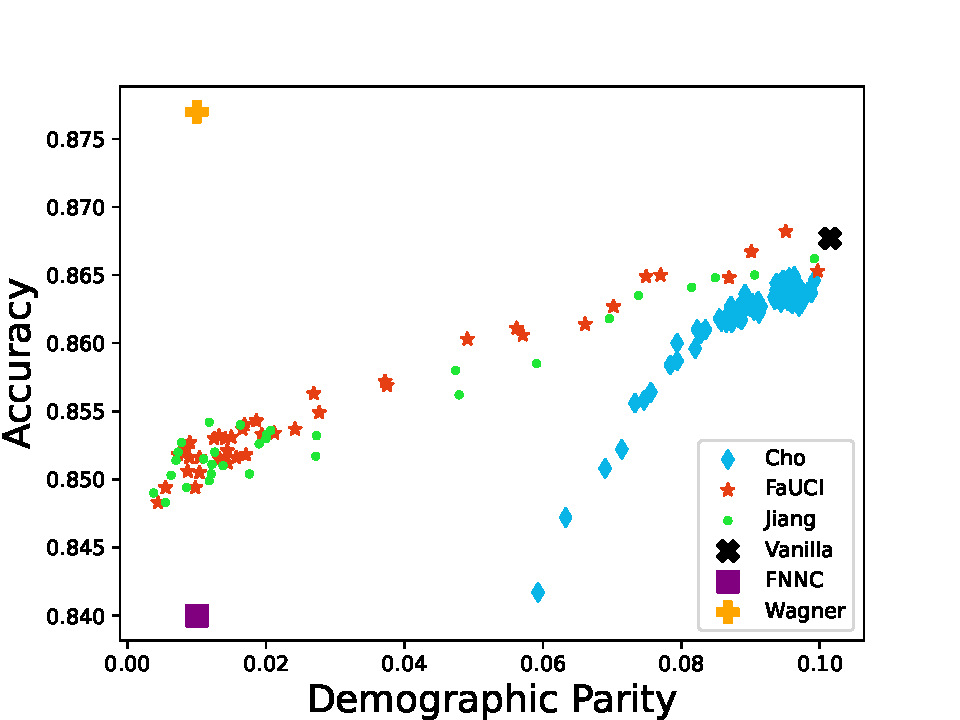
\includegraphics[width=\columnwidth]{figures/fauci/accuracy/demographic_parity_sex}
        \caption{Sensitive attribute: sex}
        \label{fig:dp-sex}
    \end{subfigure}
    %
    \begin{subfigure}[]{\onethirdsize}
        \centering
        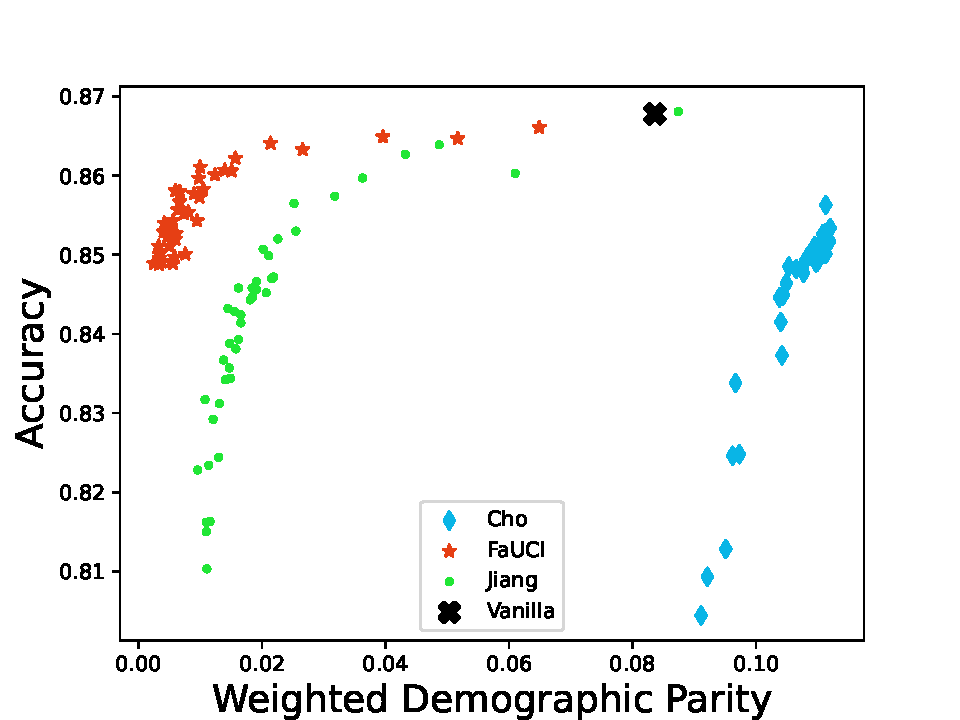
\includegraphics[width=\columnwidth]{figures/fauci/accuracy/demographic_parity_ethnicity}
        \caption{Sensitive attribute: ethnicity}
        \label{fig:dp-ethnicity}
    \end{subfigure}
    %
    \begin{subfigure}[]{\onethirdsize}
        \centering
        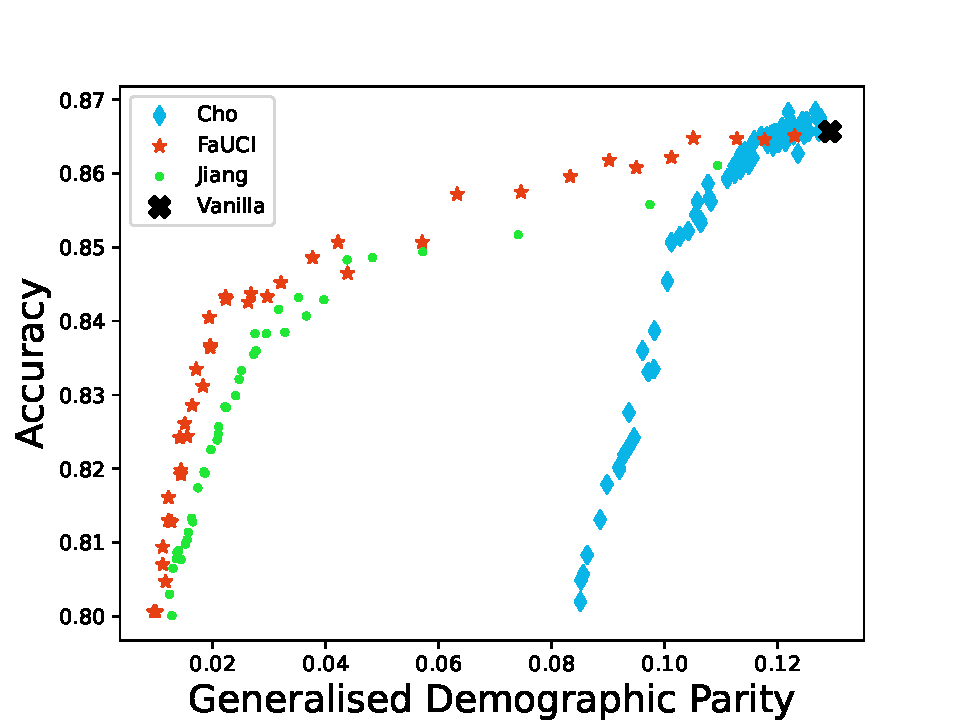
\includegraphics[width=\columnwidth]{figures/fauci/accuracy/demographic_parity_age}
        \caption{Sensitive attribute: age}
        \label{fig:dp-age}
    \end{subfigure}
    \label{fig:dp}
% \end{figure*}
% %
% \begin{figure*}[ht!]
%     \centering
%     \caption{%
%         Experiments applying DI constraints across different sensitive attributes. Legend as in \Cref{fig:dp}.
%         %
% %        Each dot is the average of 5 runs (5-folds cross-validation).
% %        %
% %        Red stars represent \fauci{}, the black cross the vanilla neural network (i.e., the NN without fairness constraints) and when possible, FNNC is represented as a purple square and Wagner's method as an orange cross.
%     }

    \begin{subfigure}[]{\onethirdsize}
        \centering
        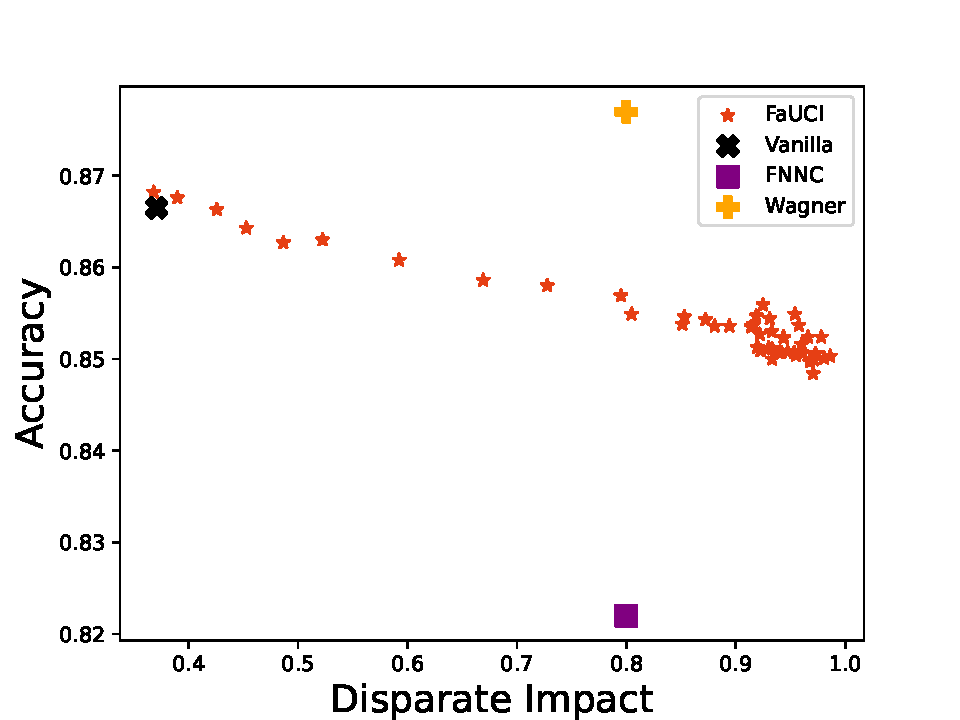
\includegraphics[width=\columnwidth]{figures/fauci/accuracy/disparate_impact_sex}
        \caption{Sensitive attribute: sex}
        \label{fig:di-sex}
    \end{subfigure}
    %
    \begin{subfigure}[]{\onethirdsize}
        \centering
        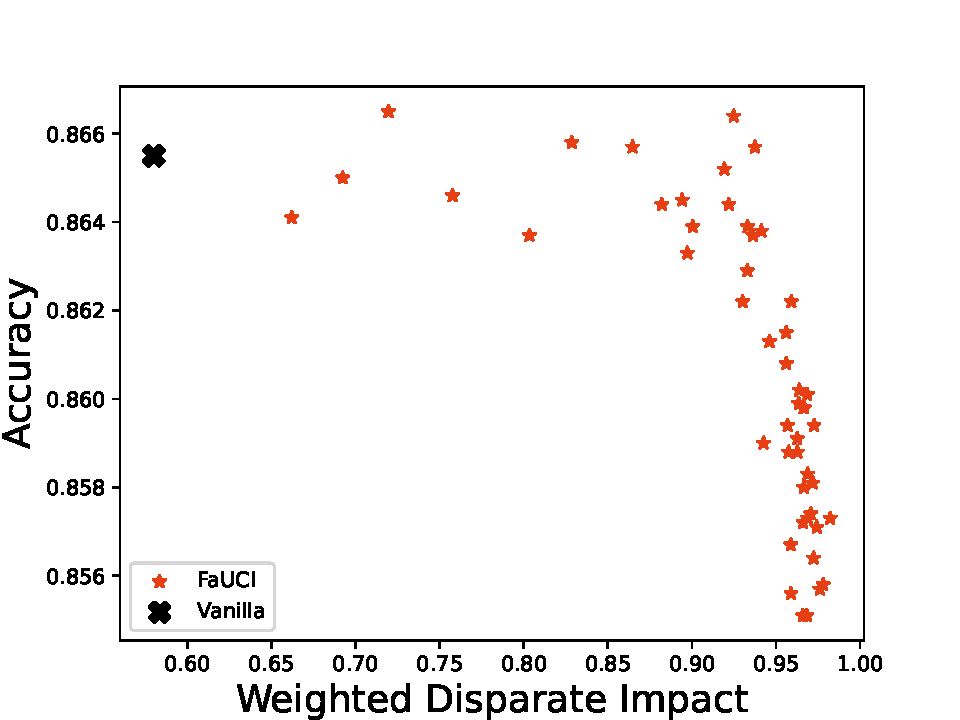
\includegraphics[width=\columnwidth]{figures/fauci/accuracy/disparate_impact_ethnicity}
        \caption{Sensitive attribute: ethnicity}
        \label{fig:di-ethnicity}
    \end{subfigure}
    %
    \begin{subfigure}[]{\onethirdsize}
        \centering
        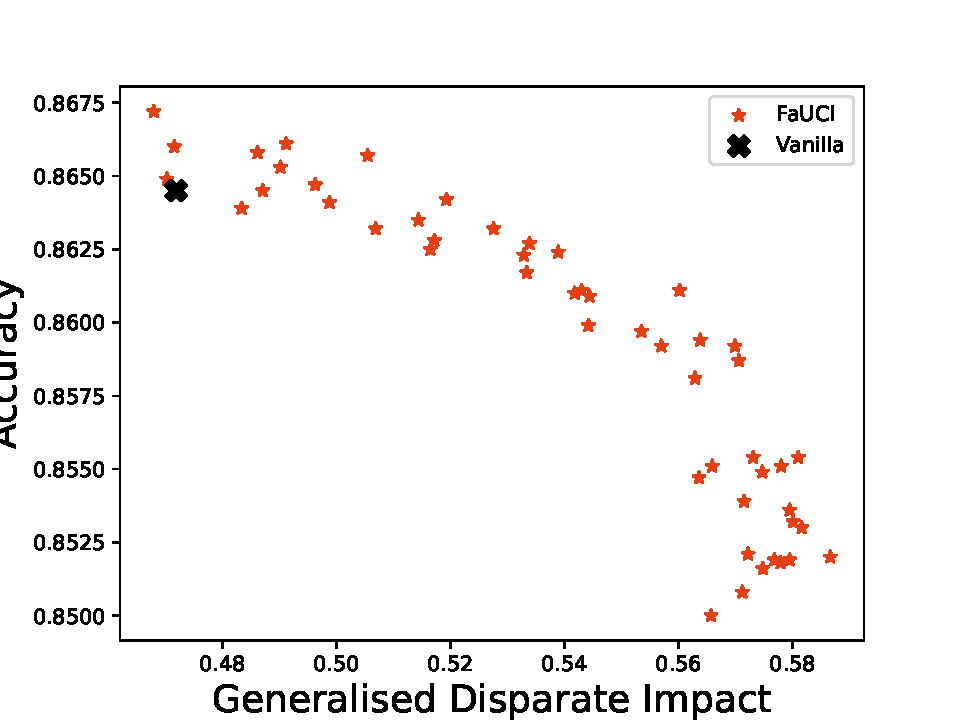
\includegraphics[width=\columnwidth]{figures/fauci/accuracy/disparate_impact_age}
        \caption{Sensitive attribute: age}
        \label{fig:di-age}
    \end{subfigure}
    \label{fig:di}
% \end{figure*}
% %
% \begin{figure*}[ht!]
%     \caption{%
%     	Experiments applying EO constraints across different sensitive attributes. Legend as in \Cref{fig:dp}.
%         %fairness methods results with different sensitive attributes.
%         %
% %        Each dot is the average of 5 runs (5-folds cross-validation).
% %        %
% %        Red stars represent our method, blue diamonds Cho's method, the black cross the vanilla neural network (i.e., the NN without fairness constraints) and when possible, FNNC is represented as a purple square.
%     }

    \begin{subfigure}[]{\onethirdsize}
        \centering
        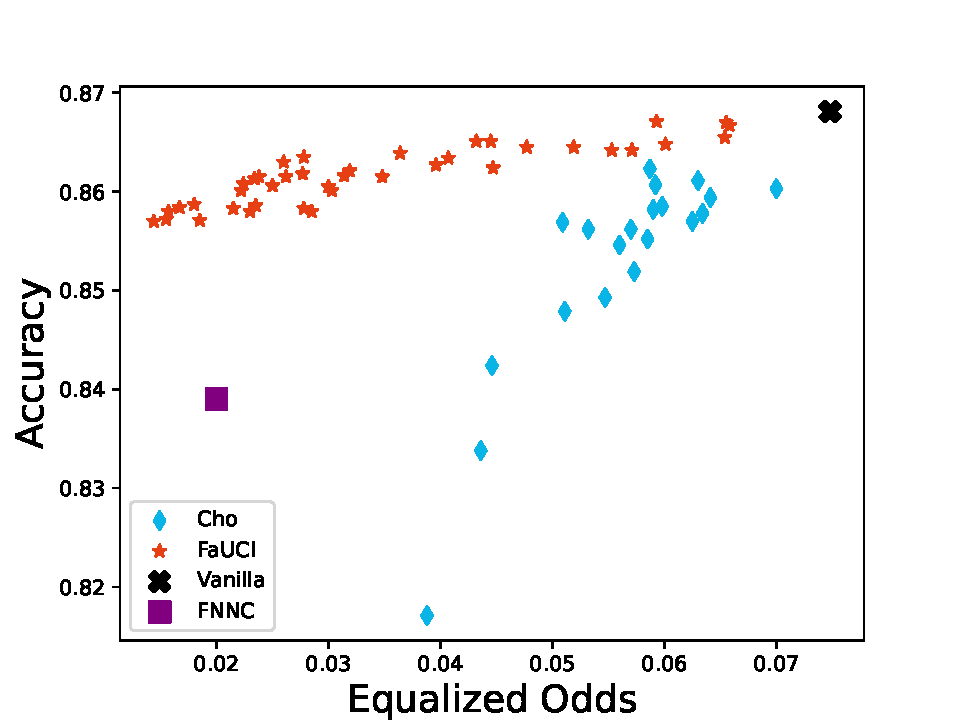
\includegraphics[width=\columnwidth]{figures/fauci/accuracy/equalized_odds_sex}
        \caption{Sensitive attribute: sex}
        \label{fig:eo-sex}
    \end{subfigure}
    %
    \begin{subfigure}[]{\onethirdsize}
        \centering
        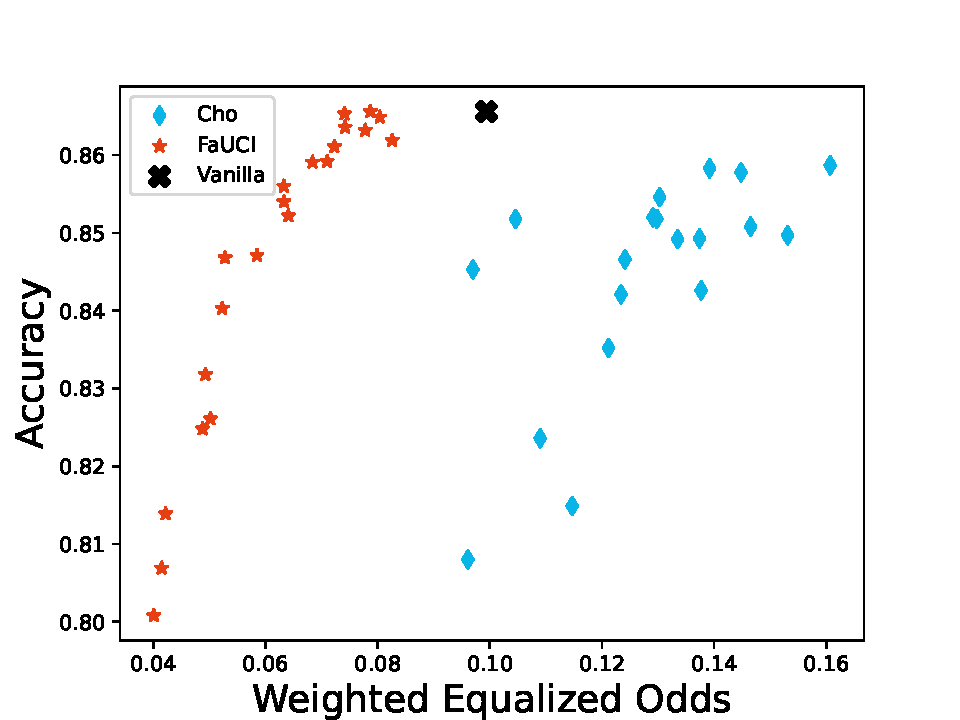
\includegraphics[width=\columnwidth]{figures/fauci/accuracy/equalized_odds_ethnicity}
        \caption{Sensitive attribute: ethnicity}
        \label{fig:eo-ethnicity}
    \end{subfigure}
    %
    \begin{subfigure}[]{\onethirdsize}
        \centering
        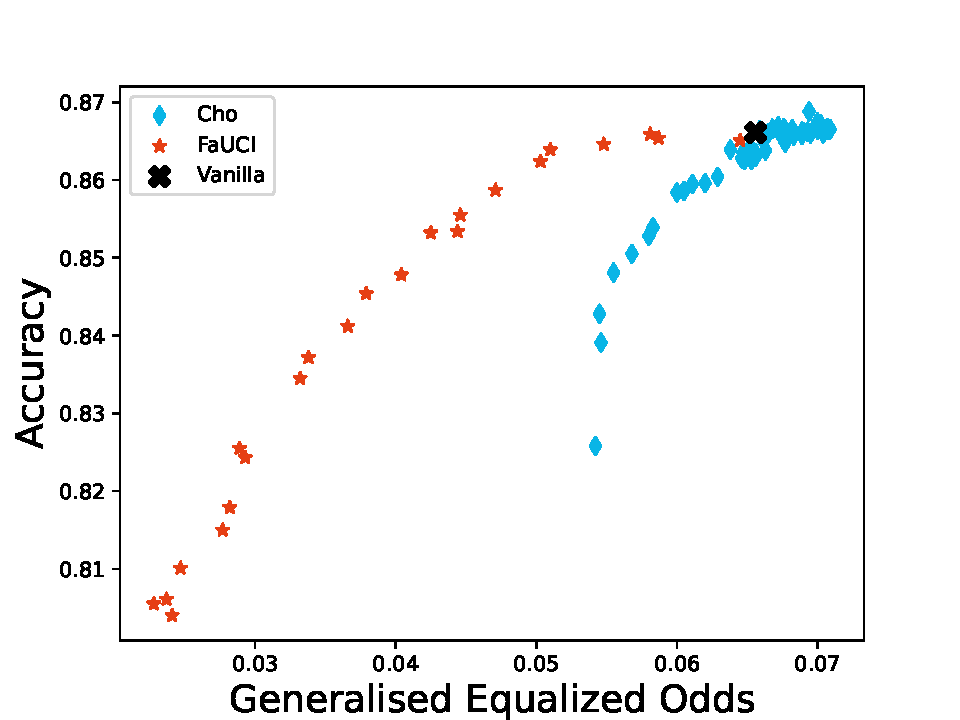
\includegraphics[width=\columnwidth]{figures/fauci/accuracy/equalized_odds_age}
        \caption{Sensitive attribute: age}
        \label{fig:eo-age}
    \end{subfigure}
    \label{fig:eo}
\end{figure}
%
\note{Update and improve the figures}
%
\paragraph{Demographic Parity Results}
%
\Cref{fig:dp} illustrates the trade-off between accuracy and \gls{DP} for \gls{FaUCI}, \gls{KDE}, \gls{GDP}, \gls{FNNC}, and \gls{LTN} methods.
%
For \emph{sex} as a binary sensitive attribute, \gls{FaUCI} achieves an accuracy of \(85.27\%\) with \(\text{DP} \leq 0.01\), outperforming \gls{KDE} and matching \gls{GDP}'s performance.
%
\gls{FNNC} and \gls{LTN} results are represented by single points, with accuracies of \(84\%\) and \(87.7\%\), respectively.
%
For \emph{ethnicity}, a categorical sensitive attribute, \gls{FaUCI} outperforms all methods, particularly when \(\text{DP} \leq 0.04\).
%
For \emph{age}, a continuous sensitive attribute, \gls{FaUCI} and \gls{GDP} perform similarly, but \gls{FaUCI} generally achieves better results.
%
Overall, \gls{FaUCI} demonstrates superior performance across all sensitive attributes.

%
\paragraph{Disparate Impact Results}
%
\Cref{fig:di} shows the trade-off between accuracy and \gls{DI}.
%
For \emph{sex}, \gls{FaUCI} achieves \(\text{DI} \geq 0.8\) with an accuracy of \(85.6\%\), surpassing \gls{FNNC} (\(82.2\%\)) and matching \gls{LTN} (\(87.7\%\)).
%
For \emph{ethnicity}, \gls{FaUCI} maintains the accuracy of the uneducated model (\(86.8\%\)) while achieving \(\text{DI} \geq 0.8\).
%
For \emph{age}, \gls{FaUCI} improves \(\text{DI}\) to \(0.58\) with an accuracy of \(85.5\%\), though it does not reach the desired threshold of \(0.8\).
%
These results highlight \gls{FaUCI}'s ability to enhance \gls{DI} while preserving high accuracy.

%
\paragraph{Equalized Odds Results}
%
\Cref{fig:eo} presents the trade-off between accuracy and \gls{EO}.
%
For \emph{sex}, \gls{FaUCI} achieves \(\text{EO} \leq 0.02\) with an accuracy of \(\geq 85.9\%\), outperforming \gls{KDE} and \gls{FNNC} (\(83.9\%\)).
%
For \emph{ethnicity}, \gls{FaUCI} maintains high accuracy while reducing \gls{EO}, whereas Cho's accuracy drops significantly.
%
For \emph{age}, \gls{FaUCI} outperforms \gls{KDE} in both accuracy and \gls{EO}.
%
Overall, \gls{FaUCI} demonstrates consistent improvements in \gls{EO} while preserving a favorable accuracy-fairness trade-off.
